\documentclass{ludis} % pieejams https://github.com/rihardsk/LU-nosl-guma-darbs---LaTeX

% xelatex
\usepackage{fontspec}
\usepackage{xunicode}
\usepackage{xltxtra}

%\usepackage[utf8]{inputenc}

\usepackage[]{hyperref}
\hypersetup{
    colorlinks=false
}
\urlstyle{same}

% languages
\usepackage{fixlatvian}
\usepackage{polyglossia}
\setdefaultlanguage{latvian}
\setotherlanguages{english,russian}

% fonts
%\setmainfont[Mapping=tex-text]{Times New Roman}
%\defaultfontfeatures{Scale=MatchLowercase,Mapping=tex-text}

% bibliography
%\usepackage{csquotes}
\usepackage[
    backend=biber,
    style=numeric-comp,
    sorting=none,
    natbib=true,
    url=false,
    doi=true%,
    %eprint=false
]{biblatex}
\addbibresource{bibliography.bib}

% toc
\setcounter{secnumdepth}{3}
\setcounter{tocdepth}{3}

%tables
\usepackage{longtable}

%papildus matemātika
\usepackage[showonlyrefs]{mathtools}
\newenvironment{thmenum}
 {\begin{enumerate}[label=\upshape(\arabic*),ref=\thethm(\arabic*)]}
 {\end{enumerate}}
\usepackage{amsmath}
 
%\begin{thmenum}
%\item \label{foo} Foo
%\item \label{bar} Bar
%\item \label{baz} Baz
%\end{thmenum}

%images
\usepackage{graphicx}
\usepackage{float}

%dalīšana kolonnās
\usepackage{multicol}

%saraksti
\usepackage{enumitem}

\fakultate{Datorikas}
\nosaukums{Neironu tīkli un nepārtrauktas darbību telpas Markova izvēles procesi}
\darbaveids{Maģistra kursa}
\autors{Rihards Krišlauks}
\studapl{rk09006}
\vaditajs{Prof., Dr. comp. Valdis Zuters}
%\recenzents{Juris Vīksna profesors Dr.sc.comp.}
\vieta{Rīga}
\gads{2015}

\begin{document}
\maketitle

\begin{abstract-lv}
Abstract-lv
\keywords{atslēgas vārds 1, atslēgas vārds 2}
\end{abstract-lv}
\clearpage

\begin{abstract-en}
Abstract-en
\keywords{Keyword 1, keyword 2}
\end{abstract-en}


\tableofcontents

\specnodala{Apzīmējumu saraksts}
\setlength\LTleft{0pt}
\setlength\LTright{0pt}
\begin{longtable}{| c | p{28em} |}
  \hline
  \textbf{Apzīmējums} & \textbf{Atšifrējums}\\ 
  \endhead

  \hline
  $D_X \in \mathbb{N}_+$ & \\
  $S \subseteq \mathbb{R}^{D_S}$ & \\
  $A \subseteq \mathbb{R}^{D_A}$ & \\
  $R:S \times A \times S \rightarrow \mathbb{R}$ & \\
  $T:S \times A \times S \rightarrow [0,1]$ & Apzīmējuma nosaukums \\
  $\pi(s, a)$ &  Apzīmējuma nosaukums 2\\
  \hline
\end{longtable}

\specnodala{Ievads}
Te ir ievads
\chapter{Markova izvēles procesi} \label{chap:mdp}
Nodaļā tiek apskatīti Markova izvēles procesi ar mērķi sniegt vispārīgu priekšstatu par tēmu.
Tiek doti arī piemēri un paņēmieni, kas tieši neattiecas uz darba mērķi, bet doti, lai vieglāk izprast jēdziena kontekstu, tomēr lielākā daļa izklāsta ir pozicionēta tieši vēlāk apskatāmās stimulētās mācīšanās kontekstā.

Markova izvēles procesi (angliski Markov decision processes, turpmāk tekstā - MDP) formalizē un ļauj modelēt izvēles veikšanas procesu apstākļos, kur darbības rezultāts ir atkarīgs tikai no sistēmas pašreizējā stāvokļa, bet ir daļēji nejaušs, t.i., izvēles veicējs procesu kontrolē tikai daļēji.
Mērķis ir kontrolēt sistēmu tā, lai tiktu maksimizēta kāda metrika, kas ir atkarīga no katrā solī veiktās darbības rezultāta.
Tiek uzskatīts, ka MDP ir ieviesti \autocite{Bel}.

MDP vispārina MI (mākslīgā intelekta) plānošanas paradigmu \autocite{Hendler1990ai}.
Tie ļauj plānošanas problēmu modelī iekļaut nejaušību, kas saistīta ar darbību izpildi, un ļauj specificēt mazāk konkrētus plāna mērķus.
Turklāt MDP ļauj formalizēt sistēmas, kuru darbībā jāņem vērā resursu patēriņš.
Plāns MI plānošanas izpratnē kā soļu virkne, kas paredzēta, lai no sākuma stāvokļa sasniegtu uzdoto beigu stāvokli, MDP formālismā tiek vispārināts par stratēģiju, jeb funkciju, kas katram sistēmas stāvoklim piekārto optimālo darbību, tā lai sistēmas kontroles procesā tiktu maksimizēta kāda no uzdevuma atkarīga metrika.

\autocite{Otterlo} tiek dots piemērs tipiskai MI plānošanas problēmai. Var iedomāties, ka ir dota kāda telpa ar tajā sakrāmētām kastēm, un uzdevums ir kastes pārkrāmēt tā, lai dažas no tām pārliktu norādītās vietās.
Šo uzdevumu var risināt ar MI plānošanas metodēm.
Toties, ja tiek apskatīta situācija, kur kastu krāmēšanas operators, piemēram, robots, darbības neizpilda pilnīgi precīzi, bet var pieļaut kļūdas, vai arī var iestāties kādi citi apstākļi, kas nav operatora kontrolē, tad šādam uzstādījumam dabīgāk atbilst MDP paradigma, kurā var, teiksim, uzdevuma mērķi atslābināt un teikt, ka uzdevuma mērķis ir maksimizēt atalgojumu, kas saņemts par katras kastes nolikšanu vietā.

Pieeju MDP risināšanai vada par sistēmu pieejamās informācijas veids.
Gadījumus, kad par sistēmu pieejamā informācija ir pilnīga, t.i., ir zināma sistēmas stāvokļu pāreju dinamika, kā arī ar darbību veikšanu saistītā atalgojumu funkcija, parasti mēdz risināt ar dinamiskās programmēšanas metodēm.
Savukārt, grūtāko uzstādījumu, kur par sistēmu nav zināma nekāda sākotnējā informācija, un informācija par sistēmas pārejām un atalgojumiem ir noskaidrojama tikai ar to mijiedarbojoties, risina ar stimulētās mācīšanās metodēm, kas tiek apskatītas šajā darbā.

Tālāk tiek ieviesta Markova izvēles procesu definīcija. Mēs lietosim definīciju, kas pieļauj nepārtrauktas stāvokļu un darbību telpas. Ievērosim, ka definīciju var sašaurināt uz diskrētām stāvokļu vai darbību telpām, ņemot $S \subseteq \mathbb{N}^{D_S}$ vai $A \subseteq \mathbb{N}^{D_A}$.

\begin{definicija}
Par Markova izvēles procesu, jeb MDP, sauc kortežu $(S, A, T, R)$, kur:
\begin{itemize}
	\item $S \subseteq \mathbb{R}^{D_S}$, kur $D_S \in \mathbb{N}$, ir stāvokļu kopa, %TODO iespējams bezgalīga?
	\item $A \subseteq \mathbb{R}^{D_A}$, kur $D_A \in \mathbb{N}$, ir darbību kopa, %TODO iespējams bezgalīga?
	\item $T:S \times A \times S \rightarrow [0,1]$ ir pārejas funkcija, kur $T(s, a, s')$ norāda varbūtību, esot stāvoklī $s \in S$ veicot darbību $a \in A$, nonākt stāvoklī $s' \in S$,
	\item $R:S \times A \times S \rightarrow \mathbb{R}$ ir atalgojuma funkcija, $R(s, a, s')$ norāda atalgojumu, kas tiek saņemts, esot stāvoklī $s \in S$ veicot darbību $a \in A$ un pēc tam nonākot stāvoklī $s' \in S$.
\end{itemize}
Ja stāvokļu telpa ir nepārtraukta, $T(s, a, s')$ apzīmē varbūtību blīvuma funkciju, jeb
\[
	\int_{S'} T(s, a, s')ds' = P(s_{t+1} \in S' \mid s_t = s \land a_t = a),
\]
kas norāda varbūtību, ka stāvoklī $s \in S$, veicot darbību $a \in A$ pāreja beigsies stāvoklī, kas pieder apgabalam $S'$. %TODO jāpaskaidro _t un _{t+1}?
\end{definicija}
%TODO beigu stāvokļi?

MDP definīcijā mēdz arī iekļaut atlaides koeficientu (angliski discount factor), ko apzīmē ar $\gamma \in [0,1]$.
Tas raksturo to, kā atšķiras nākotnē saņemtie no tagadnē saņemtajiem atalgojumiem.
Šajā darbā tiek pieņemts, ka $\gamma$ pieder pie katra konkrētā algoritma specifikācijas. %TODO šis vārds izbīdāš aiz paragrāfa malas robežas
Tas tiek darīts tādēļ, ka $\gamma$ divi dažādi algoritmi vienā un tajā pašā uzdevumā var sniegt dažādus rezultātus pie dažādām $\gamma$ vērtībām, %TODO vajag atsauci
tāpēc $\gamma$ izvēle tiek atstāta algoritma ziņā, tā kā tā maiņā neietekmē uzdevuma būtību. %TODO ok, šīs varbūt ir muļķības. ko darīt, ja gamma ir līdzeklis, ar ko specificēt kādu uzdevumam noderīgu aspektu?
Šādā veidā MDP tiek ieviesti arī \autocite{Otterlo}.

Parasti tiek ieviesta arī funkcija $\pi: S \times A \rightarrow [0, 1]$, kas apzīmē optimālo stratēģiju, jeb kontroles shēmu:
\[
	\pi(s, a) = P(a_t = a \mid s_t = s),
\]
kur $\sum_{a\in A} \pi(s,a)=1$, ja darbību telpa ir diskrēta, un $\int_{A} \pi(s,a) da = 1$, ja tā ir nepārtraukta. Funkcija norāda varbūtību, ar kādu optimālajā stratēģijā esot stāvoklī $s \in S$ tiek veikta darbība $a \in A$. Gadījumā, ja darbību telpa ir nepārtraukta, $\pi$ ir varbūtību blīvuma funkcija.

Neformāli to var iedomāties (no stimulētās mācīšanās pieejas skatpunkta) kā procesu, kur darbību veicējs, sauksim viņu par aģentu, var novērot to, kādā 
stāvoklī sistēma ir pašlaik, un viņam ir pieejama informācija par darbībām, ko ir iespējams veikt.
Aģents izvēlas darbību un novēro jauno stāvokli, uz kuru pāriet sistēma, kā arī rezultātā saņemto atalgojumu.
Aģenta mērķis ir izvēlēties darbības tā, lai maksimizētu laika gaitā saņemto atalgojumu.
Aģents iepriekš nezina ne varbūtību, ar kādu tiks veikta viņa izvēlētā pāreja, ne pašu stāvokli, uz kuru pāries sistēma, ne arī atalgojumu, ko saņems.
Šo informāciju viņam ir jāuzkrāj laika gaitā no iepriekšējās pieredzes.

Jāņem vērā, ka uzdevumu sarežģī tieši iepriekš minētā nenoteiktība.
Sākot darbu, aģentam iepriekš nezināmā domēnā, tam trūkst jebkādas informācijas par uzdevumu, un tā ir iegūstama tikai mijiedarbojoties ar domēnu.
Turklāt par izdarītās izvēles labumu liecina nevis uzreiz pēc tās veikšanas saņemtais atalgojums, bet gan arī atalgojums, kas saņemts nākotnē, pēc šī stāvokļa apmeklēšanas.
Citiem vārdiem -- darbības izdevīgums ir jāvērtē ilgtermiņā.
Vēl viens aspekts, kura nozīme pieaug jo īpaši nepārtrauktās stāvokļu un darbību telpās, ir soļu skaits, pēc kura aģents atrod stratēģiju, kas tuva optimālajai.
Ja pārtrauktās, galīgās stāvokļu telpās vēlme ir, lai, meklējot optimālo stratēģiju katrs stāvoklis tiktu apmeklēts pēc iespējas mazāk reižu, tad nepārtrauktās stāvokļu un darbību telpās katru stāvokli un darbību nemaz nav iespējams izmēģināt, tā kā to skaits ir neierobežots.
Šis apsvērums nošķir stratēģijas, kas izmantojamas MDP risināšanas algoritmā. %TODO laikam slikti skan. jāpārformulē

%TODO jāievieš stāvokļu-darbību vērtības funkcija

%TODO jāievieš stāvokļu vērtības funkcija

%TODO jāpasaka, kas ir Belmana vienādojumi, varbūt

Jāpiebilst, ka tie paši apsvērumi, kas šajā nodaļā ir izteikti par nepārtrauktām stāvokļu un darbību telpām, lielā mērā ir attiecināmi arī uz diskrētām, bet lielām telpām.
Turpmākajā tekstā, runājot par diskrētām telpām, domātas ir telpas, kuras ir pietiekami mazas.
Konkrēti apmēri šeit netiek minēti, jo tie atkarīgi no pieejamajiem skaitļošanas resursiem.

\section{Stratēģijas optimalitāte}
Darbā jau vairākkārt ir pieminēts, ka stratēģijai, kas tiek izmantota MDP kontrolē jāapmierina kaut kādus optimalitātes kritērijus.
Izteiksim šo prasību formālāk, norādot trīs iespējamos optimalitātes kritērijus, kā tie ieviesti \autocite{Otterlo}.

\begin{definicija}
Teiksim, ka dotam MDP, ko apzīmēsim ar $M$, stratēģija $\pi$ ir optimāla galīgā horizonta nozīmē, ja tā maksimizē izteiksmi:
\[
	E\left[\sum_{t=0}^{h}r_t\right],
\]
kur $h \in \mathbb{N}$ ir horizonta izmērs, un $r_t$ apzīmē $t$-ajā solī saņemto atalgojumu, kontrolējot $K$ pēc shēmas $\pi$.
\end{definicija}

\begin{definicija}
Teiksim, ka dotam MDP, ko apzīmēsim ar $M$, stratēģija $\pi$ ir optimāla bezgalīgā horizonta nozīmē, ja tā maksimizē izteiksmi:
\[
	E\left[\sum_{t=0}^{\infty}\gamma^t r_t\right],
\]
kur $\gamma \in \left[0, 1\right)$ ir atlaides koeficients, un $r_t$ apzīmē $t$-ajā solī saņemto atalgojumu, kontrolējot $K$ pēc shēmas $\pi$.
\end{definicija}

\begin{definicija}
Teiksim, ka dotam MDP, ko apzīmēsim ar $M$, stratēģija $\pi$ ir optimāla vidējā atalgojuma nozīmē, ja tā maksimizē izteiksmi:
\[
	\lim\limits_{h \rightarrow \infty} E\left[\frac{1}{h}\sum_{t=0}^{h}r_t\right],
\]
kur $h \in \mathbb{N}$ ir horizonta izmērs, un $r_t$ apzīmē $t$-ajā solī saņemto atalgojumu, kontrolējot $K$ pēc shēmas $\pi$.
\end{definicija}

Optimalitātes kritērija izvēle var būt atkarīga no risināmās problēmas. Pārskats par dažādu optimalitātes kritēriju izmantošanu MDP modelēšanā ir dots \autocite{koenig2002interaction}.
Turpmāk tekstā tiks izmantots bezgalīgā horizonta optimalitātes nosacījums.

%TODO svarīgi, pārskata grāmata saka, ka kritērijus ar konkrētu \pi sasaista value funkcija. es savukārt neredzu iemeslu, kāpēc mest \pi no definīcijas laukā

\section{Vērtības funkcija un stāvokļu-darbību vērtības funkcija}
Stāvokļu vērtības funkcija, vai vienkāršāk -- vērtības funkcija -- tiek ieviesta, lai izteiktu stāvokļa vērtību pie konkrētas stratēģijas.
Tā izsaka, cik izdevīgi ir atrasties kādā stāvoklī pie dotās stratēģijas, ņemot vērā optimalitātes nosacījumu.
\begin{definicija}
Teiksim, ka ir dota kontroles shēma $\pi$.
Tai atbilstošā stāvokļu vērtības funkcija $V^\pi : S \rightarrow \mathbb{R}$ izsaka sagaidāmo atalgojumu, sekojot stratēģijai $\pi$, sākot no stāvokļa $s$:
\[
	V^\pi (s) = E_\pi \left\{ \sum_{k=0}^{\infty} \gamma^k r_{t+k} \mid s_t = s\right\}
\]
\end{definicija}

Līdzīgi var ieviest arī stāvokļu-darbību vērtību funkciju:
\begin{definicija}
Teiksim, ka ir dota kontroles shēma $\pi$.
Tai atbilstošā stāvokļu-darbību vērtības funkcija $Q^\pi : S \times A \rightarrow \mathbb{R}$ izsaka sagaidāmo atalgojumu, sekojot stratēģijai $\pi$, sākot no stāvokļa $s$ un veicot darbību $a$:
\[
	Q^\pi (s,a) = E_\pi \left\{ \sum_{k=0}^{\infty} \gamma^k r_{t+k} \mid s_t = s \land a_t = a\right\}
\]
\end{definicija}

Tagad varam pārformulēt optimālās stratēģijas jēdzienu:
\begin{definicija}
Teiksim, ka stratēģija ir optimāla, un apzīmēsim to ar $\pi^*$, ja visiem stāvokļiem $s \in S$ un visām stratēģijām $\pi$ izpildās:
\[
	V^{\pi^*}(s) \geq V^{\pi}(s)
\]
\end{definicija}

\section{MDP risināšana un Bellmana vienādojumi}
Īsumā ieskatīsimies MDP risināšanas iespējās.
Bellmana optimalitātes vienādojums ļauj rekursīvi izteikt optimālo stāvokļu vērtības funkciju $V^* = V^{\pi^*}$ atkarībā no pārejas un atalgojuma funkcijām \autocite{Bel}\autocite{Otterlo}\autocite{Hasselt2012}.
Šeit tas ir izteikts nepārtrauktām stāvokļu telpām: 
\[
	V^*(s) = \max_{a\in A} \int_S T(s,a,s')\left(R(s,a,s') + \gamma V^*(s)\right) ds'.
\]
Vienādojums sniedz arī veidu, kā izteikt pašu optimālo stratēģiju:
\begin{equation}
	\pi^*(s) =  \arg \max_{a} \int_S T(s,a,s')\left(R(s,a,s') + \gamma V^*(s)\right) ds'. \label{eq:1}
\end{equation}
Līdzīga sakarība ir arī spēkā optimālajai stāvokļu-darbību vērtības funkcijai $Q^* = Q^{\pi^*}$:
\[
	Q^*(s, a) = \int_S T(s,a,s')\left(R(s,a,s') + \gamma \max_{a'}Q^*(s',a')\right) ds'.
\]
$Q^*$ un $V^*$ saista sakarības:
\[
	Q^*(s, a) = \int_S T(s,a,s')\left(R(s,a,s') + \gamma V^*(s')\right) ds',
\]
\[
	V^*(s) = \max_{a} Q^*(s,a),
\]
kas ļauj izteikt optimālo stratēģiju arī ar stāvokļu-darbību vērtības funkciju:
\begin{equation}
	\pi^*(s) = \arg \max_a Q^*(s, a). \label{eq:2}
\end{equation}

Augstāk redzamie vienādojumi ļauj kategorizēt veidus, kādos risināmi MDP.

\subsection{Modeļa aproksimācija}
Modeļa aproksimācijas pieejā tiek mēģināts tuvināti atrast dotās MDP nezināmos parametrus -- pāreju funkciju $T$ un atalgojuma funkciju $R$ --, lai no tām atvasinātu aproksimētās MDP optimālo kontroles shēmu.
Modeļa meklēšanā tiek pieņemts, ka kopas $S$ un $A$ ir zināmas.
Dziļākam ieskatam metodēs, kas tiek izmantotas modeļa aproksimēšanā, skatīt \autocite{nguyen2011model}.

Kad modelis ir zināms, optimālās stratēģijas atrašana galīgam stāvokļu un darbību telpām ir samērā vienkārša. Var tikt izmantots, piemēram, value iteration vai policy iteration algoritms, kam ir var pierādīt, ka tie konverģē uz optimālo $\pi^*$ \autocite{Barto}.
Tomēr vispārīgā gadījumā MDP nepārtrauktās stāvokļu telpās situācija ir krietni sarežģītāka -- katram katram stāvoklim optimālo stratēģiju atrast nav iespējams \autocite{Otterlo}.
Piemēram, iepriekš minētie value iteration un policy iteration algoritmi satur ciklu pa visu stāvokļu kopu, kas algoritmu padara nelietojamu, ja stāvokļu skaits ir bezgalīgi liels.

%TODO šo varbūt var iekļaut: Alternatīvi \autocite{Otterlo} tiek minēta iespēja tuvināto MDP izmantot, lai ģenerētu 

Lai arī iepriekš minētie argumenti nav spēkā uz MDP ar nepārtrauktām darbību telpām, autors neredz tiešu veidu, kā pieeja būtu vispārināma, lai no iegūtā MDP modeļa atvasinātu stratēģiju, kas optimālo darbību stāvoklī atrod ar neirona tīkla palīdzību.
%TODO jāpasaka, kāpēc neironu tīkls būtu labāks
Turklāt, lai arī kā darba mērķis netika uzstādīta prasība algoritmam darboties arī ar nepārtrauktām stāvokļu telpām, nevajadzīga algoritma vispārīguma samazināšana, ja no tā var izvairīties, tiek uzskatīta par nevēlamu.

\subsection{Vērtību aproksimācija}
Vērtību aproksimācijas piegājienā tiek nevis mēģināts atrast trūkstošās pāreju un atalgojuma funkcijas, bet gan tiek uzreiz mēģināts tuvināti atrast funkcijas $V^*$ vai $Q^*$.
Kā redzams iepriekšējā sadaļā, vienādojumi \eqref{eq:1} un \eqref{eq:2} ļauj atrast $\pi^*$, ja $V^*$ vai $Q^*$ ir zināma.
Šīs kategorijas algoritmus iedala atkarībā no tā, vai tie ir spējīgi mācīties tiešsaistē, un vai algoritms ir on-policy vai off-policy tipa.

Atsaucoties uz \autocite{Hasselt2012} -- on-policy algoritmi mēģina tuvināti atrast stāvokļu vērtības funkciju $V^\pi$ vai stāvokļu-darbību vērtības funkciju $Q^\pi$ stratēģijai $\pi$, kura konkrētajā brīdī tiek izmantota.
Lai arī optimālā stratēģija $\pi^*$ iesākumā nav zināma, on-policy algoritmi pakāpeniski nonāk pie optimālās funkcijas $V^{\pi^*}$ vai $Q^{\pi^*}$, iteratīvi katrā solī uzlabojot sev zināmo $\pi$.
Off-policy tipa algoritmi izmanto citu pieeju, kas tiešā veidā necenšas atrast optimālo stratēģiju $\pi^*$.
Funkciju $V^{\pi^*}$ vai $Q^{\pi^*}$ novērtējumi var tikt uzlaboti, sekojot stratēģijām, kas nav optimālas.

Algoritmus, kas spējīgi mācīties tiešsaistē, jeb online algoritmus, raksturo tas, ka tie savus novērtējumus pielāgo pēc katras pārejas veikšanas, novērojot jauno sistēmas stāvokli un saņemto atalgojumu.
Pretnostatījumā offline algoritmi ieejas datus apstrādā pa vairākiem novērojumiem vienā grupā.
Online algoritmiem ir raksturīgas mazākas prasības pēc skaitļošanas resursiem viena novērojuma apstrādāšanai. Tie strādā labi gadījumos, kad novērojumu ir pieejams daudz un viena novērojuma veikšana nav resursietilpīga.
Offline algoritmi savukārt efektīvāk izmanto pieejamos novērojumus, kas tiem ļauj līdzvērtīgu rezultātu sasniegt, apstrādājot mazāk novērojumu.

Pie on-policy algoritmiem pieder, piemēram, temporal-difference saimes algoritmi. Pie off-policy algoritmiem pieskaitāms, piemēram, ir Q-learning un tā varianti. Katrā minēto algoritmu grupā ietilpst gan online, gan offline algoritmu varianti \autocite{Barto}.

Minētajiem algoritmiem darbošanās nepārtrauktās stāvokļu telpās nesagādā problēmas. Šādās situācijās parasti $V^{\pi^*}$ vai $Q^{\pi^*}$ reprezentācijai tiek izmantota kāda funkciju aproksimēšanas pieeja, piemēram, neironu tīkli. Kā piemēru var skatīt \autocite{tesauro1995temporal}, kur neironu tīkls tiek trenēts ar Q-learning, lai aproksimētu funkcijas $Q^{\pi^*}$ vērtību backgammon spēlē.
Jaunākā avotā \autocite{mnih2013playing} Q-learning variants tiek izmantots, lai autonomi apmācītu aģentu spēlēt vairākas Atari 2600 videospēles, kā ieejas datus izmantojot tikai spēlēs ekrāna pikseļu vērtības (bez īpašas priekšapstrādes) un spēles rezultātu.
$Q^{\pi^*}$ aproksimēšanai tiek izmantots neironu tīkls.
Šis rezultāts ir īpaši interesants, jo spēles stāvokļu telpa ir izteikti sarežģīta, lai no spēles ekrāna pikseļu vērtībām būtu iespējams kaut ko pateikt par pašreizējo spēles stāvokli, aģentam ir jāiemācās pikseļu vērtības abstrahēt sarežģītākos objektos.
To šeit paveic neironu tīkls.

Ar nepārtrauktām darbību telpām ir citādi.
Tā kā bieži šajos algoritmos, lai atrastu optimālo stratēģiju, atbilstoši \eqref{eq:2} tiek meklēts atrisinājums izteiksmei
\[
	\arg \max_a Q^*(s, a),
\]
tad nevar iztikt bez darbību telpas diskretizēšanas.
Literatūrā un praksē sastopami dažādi diskretizācijas varianti -- sākot no vienkāršākajiem kā tile coding, kur darbību telpa tiek sadalīta nepārklājošos apgabalos, kas katrs uztverams kā diskretizētās darbību telpas atsevišķs elements, līdz sarežģītākām, kā, piemēram, Kanerva coding \autocite{Barto}.

Algoritmus, kuros optimālā stratēģija tiek atvasināta no $Q^*$ funkcijas, kā redzams augstāk, grūti vispārināt atbilstoši darba mērķim darbībai ar neironu tīkliem, jo tas prasa algoritmam glabāt neironu tīkla vai kāda cita funkciju aproksimētāja svarus, un tos darbības laikā pielāgot.
Cik autoram zināms, šādas problēmas pastāv off-policy algoritmos, piemēram, minētajā Q-learning.
On-policy algoritmi šajā aspektā darba ietvaros nav pētīti.

\subsection{Stratēģijas aproksimācija}
Atšķirībā no vērtību aproksimācijas algoritmiem, stratēģijas aproksimācijas pieejas algoritmi optimālās stratēģijas tuvinājumu glabā tiešā veidā.
Parasti nav nekādu šķēršļu $\pi^*$ reprezentācijai izmantot kādu vispārīgu funkciju aproksimētāju. Tādā gadījumā algoritms glabā tā parametrus.
Šim nolūkam var tikt izmantots arī neironu tīkls.
Bez tuvinātas optimālās stratēģijas mēdz tikt glabāta arī $V^{\pi^*}$ vai $Q^{\pi^*}$ funkcija.
Algoritmus, kuros tiek tā darīts, mēdz saukt par actor-critic algoritmiem, ar vārdu critic atsaucoties uz algoritma daļu, kas vērtē spēles stāvokļa izdevību, jeb $V^{\pi^*}$ vai $Q^{\pi^*}$, un ar actor atsaucoties uz stratēģiju.
Pēc analoģijas, stratēģijas aproksimācijas algoritmus, kas neizmanto kādu no vērtību funkcijām, dēvē par actor-only algoritmie, savukārt vērtību aproksimācijas algoritmus -- par critic-only algoritmiem.
Stratēģijas aproksimācijas algoritmi tiks tuvāk apskatīti \ref{chap:stim} nodaļā.

\chapter{Funkciju aproksimācija}
Nodaļā tiek likts uzsvars uz nelineāro funkciju aproksimētāju, it īpaši neironu tīklu, apskatu, bet tiek arī apskatīti un īsumā izvērtēti citu klašu funkciju aproksimētāji, uzmanību pievēršot, piemēram, ģenētiskajiem algoritmiem.

Ar funkciju aproksimēšanu, sauktu arī par funkciju tuvināšanu, tiek saprastas pieejas, kuru mērķis ir, par izejas datiem ņemot aproksimējamās, jeb mērķa, funkcijas vērtības, atrast citu funkciju noteiktā klasē, kas pēc iespējas vairāk atbilst aproksimējamajai.
Bieži vien aproksimējamā funkcija kā tāda nemaz nepastāv, bet aproksimēšana notiek ar mērķi iegūt funkciju, kas izsaka sakarības, kas novērojamas kādā mūs interesējošā procesā.
Skatoties mašīnmācīšanās kontekstā, vai konkrētāk -- apskatot pārraudzītās mācīšanās (supervised learning) problēmu -- mērķis ir no dota datu korpusa, kas satur kāda mūs interesējoša objekta parametrus, kam attiecināta kāda no parametriem (iespējams daļēji) atkarīga vērtība, konstruēt funkciju, kas, ieejā saņemot minētā veida parametrus, būtu spējīga prognozēt iepriekš neredzētu datu punktu vērtības.

Stimulētās mācīšanās uzdevumos, kur tiek lietotas vērtību aproksimācijas pieejas, funkciju aproksimēšana tiek lietota, lai ar kādiem domēnu aprakstošiem parametriem izteiktu stāvokļu vai stāvokļu-darbību vērtību funkciju. Stratēģijas aproksimācijas pieejās funkciju aproksimācija var tikt lietota, lai izteiktu optimālo stratēģiju atkarībā no MDP stavokļa.
Funkciju aproksimācijā sakarības, kas atrastas novērotajos datos, tiek vispārinātas uz datiem, kas nav redzēti. Tas ir ļoti svarīgs ieguvums stimulētās mācīšanās problēmās ar nepārtrauktām vai ļoti lielām stāvokļu vai darbību telpām, tā kā nav nepieciešams apskatīt visus telpas punktus, lai algoritms spētu sekmīgi darboties.

Mašīnmācīšanās pieejas nav vienmēr tiešā veidā pielietojamas stimulētās mācīšanās uzdevumos.
Stimulētās mācīšanās kontekstā uzdevumu parasti papildus apgrūtina fakts, ka vērtības, kas tiek izmantotas, lai funkcijas aproksimētāja pielāgošanai, pašas ir atkarīgas no tā snieguma -- gājieni, ko veic aģents ir atkarīgi no spēles stāvokļa novērtējuma.

Nākamajās sadaļās tiks apskatītas galvenās funkciju aproksimētāju klases, lielāku uzmanību pievēršot nelineārajiem aproksimētājiem un neironu tīkliem.

\section{Funkciju aproksimēšanas veidi}
Funkciju aproksimētājus, atkarībā no to uzbūves, mēdz iedalīt lineārajos un nelineārajos. Lineārie aproksimētaji tiks apskatīti ierobežoti, vairāk uzmanības veltot nelineārajiem aproksimētājiem.
Jēdziens funkciju aproksimētājs tiek lietots, apzīmējot funkciju, kas tiek izmantota dotās mērķa funkcijas aproksimēšanai.
Piemēram, sakot "lineārs funkciju aproksimētājs" jāsaprot, ka izmantotā funkcija ir lineāra.

\subsection{Lineārā funkcju aproksimēšana}
Par lineāru funkciju dēvē tādu funkciju, ko var izteikt formā
\[
	F(\phi) = \Theta^T \phi,
\]
kur $\Theta$ ir funkcijas parametru vektors un $D_\Theta = D_\phi$.
Stimulētās mācīšanās kontekstā parasti tiek pieņemts, ka $\phi$ ir kāda funkcija parametru iegūšanai no MDP stāvokļa $\phi : S \times \Phi$, kur $\Phi$ ir kāda parametru telpa.
Tad, lineāru funkciju izmantojot, piemēram, stāvokļu vērtības funkcijas aproksimēšanai, to var izteikt formā
\[
	V(s) = \Theta^T \phi(s).
\]
Jāpiemin, ka nosacījums, ka stāvokļu vērtības funkcija ir izsakāma kā lineāra kombinācija no parametru vērtībām, nenozīmē, ka tai jābūt lineārai attiecībā pret stāvokļu telpu.
Izvēloties pazīme, kas nav lineāras attiecībā pret stāvokļu telpu, tiek iegūta nelineāra stāvokļu vērtības funkcija attiecībā pret $S$.

Kā redzams, gadījumā, kad stāvokļu telpa ir nepārtraukta, funkcija $\phi$ to attēlo uz galīgu skaitu elementu.
Citiem vārdiem -- stāvokļu telpa tiek diskretizēta.
Pats veids, kā notiek pazīmju piekārtošana stāvokļiem nosaka diskretizācijas veidu.
Piemēram, ja stāvokļu telpa tiek sadalīta vienādos apgabalos, kam katram tiek piekārtota sava unikāla pazīme, tad iegūto attēlojumu sauc par tile coding, kas tika minēts jau iepriekš.

Lineārajiem funkciju aproksimētājiem nepārtrauktās telpās piemīt iepriekšējā sadaļā minētā īpašība par novērojumu vispārināšanu iepriekš neapskatītiem telpas punktiem.
Tomēr stāvokļu un darbību telpas diskretizācija ir iemesls, kāpēc šajā darbā priekšroka tiek dota tādiem nelineārajiem funkciju aproksimētājiem kā neironu tīkli.
Labākā telpas diskretizācijas pieeja var būt atkarīga no uzdevuma.
Tas ir pretrunā ar vēlmi atrast pēc iespējas vispārīgu pieeju simulētās mācīšanās uzdevumu risināšanai nepārtrauktās telpās.
Turklāt lineāriem funkciju aproksimētājiem ir citas problēmas, ar kurām var ar dažādiem panākumiem cīnīties, kas vairāk aprakstītas \autocite{Hasselt2012} .

\subsection{Neironu tīkli un nelineārā funkciju aproksimēšana}
Neironu tīkli pieder pie nelineārajiem funkciju aproksimētājiem.
Tie it veidoti uz līdzību pamata ar bioloģisko neironu tīkliem smadzenēs un parasti tiek formulēti kā savstarpēji savienotu "neironu" sistēma, kas dotus ieejas datus pārvērš izejas datos atbilstoši sistēmas neironu svariem.
Katru neironu raksturo svaru komplekts, kas ir koeficienti dotā neirona ieejas neironu vērtībām.
Neirons izejā dod ieejas neironu signālu un svaru lineāru kombināciju, kam pielietota kāda (parasti) nelineāra funkcija. To dēvē par aktivācijas funkciju.
Praksē bieži tiek lietota t.s. simgoid funkcija
\[
	f(x) = \frac{1}{1 + e^{-x}}.
\]
Izsakot to atkarībā no neirona svaru vektora $\Theta$, iegūst
\[
	f_\Theta(x) = \frac{1}{1 + e^{-\Theta^T x}},
\]
kur $D_\Theta = D_x$. Formāli neironu tīkls ir parasta parametrizējama funkcija, bet šāds skatījums ir intuitīvi vieglāk saprotams.

\begin{figure}
	\centering
	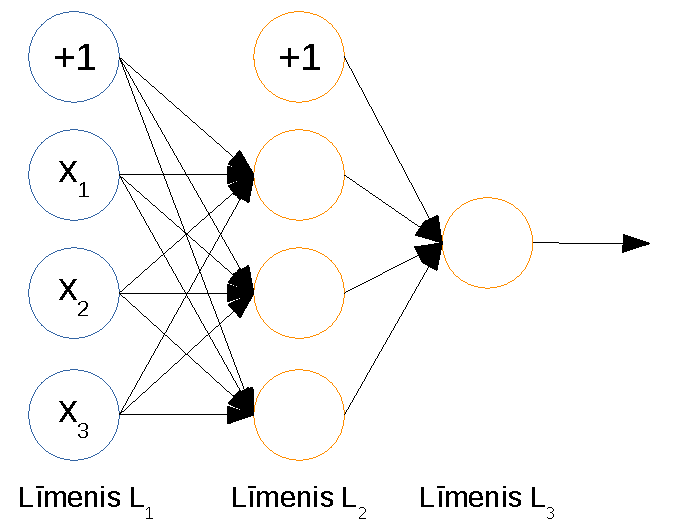
\includegraphics{Img/nn-arhitektura.pdf}
	\caption{Neironu tīkla arhitektūras piemērs.}
	\label{fig:nn}
\end{figure}

Viena no iespējamajām neironu tīklu arhitektūrām ir apskatāma attēlā \ref{fig:nn}
Šeit līmeni $L_1$ sastāda ieejas neironi, kas apzīmē tīklam padotās ieejas parametru vērtības.
Līmeni $L_3$ sastāda neironi (vispārīgā gadījumā tie var būt vairāki), kuru izejas vērtības tiek atgrieztas kā rezultāts.
Pārējos līmeņus, šoreiz tāds ir tikai viens -- $L_2$ --, sauc par slēptajiem līmeņiem.
Ar $+1$ tiek apzīmēti neironi, kas nesaņem ieejā citu neironu vērtības; tie atgriež konstanti $1$, un ļauj neironu vērtību un svaru lineārajā kombinācijā pieskaitīt koeficientu, kas nav atkarīgs no ieejas vērtībām.
Bultiņas apzīmē, kuru neironu atgrieztās vērtības tiek izmantotas kāda neirona ieejā.

Ir pierādīts, ka neironu tīkli darbojas kā universāli funkciju aproksimētāji \autocite{hornik1991approximation}.
Šo apgalvojumu formulē kā universālās aproksimācijas teorēmu (universal approximation theorem).
Tā apgalvo, ka feed-forward tipa neironu tīkls (tāds, kas atbilst \ref{fig:nn} attēla aprakstam) ar vienu slēpto slāni, ar galīgu skaitu neironu un nelineāru aktivācijas funkciju ir spējīgs aproksimēt nepārtrauktas funkcijas vērtībām, kas pieder kādai kompaktai $\mathbb{R}^n, n \in \mathbb{N}$ apakškopai.
Tas nozīmē, ka neironu tīkls ar pietiekamu ir izmantojams patvaļīgu funkciju aproksimēšanai.
Šī ir nozīmīga priekšrocība, salīdzinot ar, piemēram, lineārajiem funkciju aproksimājiem.
Turklāt, kā ieejas parametrus iespējams izmantot MDP stāvokļu mainīgos, izvairoties no atsevišķas parametru funkcijas ieviešanas.

Tomēr universālās aproksimācijas teorēma nerisina jautājumu par attiecīgo parametru algoritmisku iegūšanu, bet tikai par to eksistenci.
Praksē uzdevums vispārīgā gadījumā ir sarežģīts.
Neironu tīkla parametru iegūšanu apgrūtina nepieciešamība izvairīties no lokālajiem minimumiem trenēšanas procesā, tīkla arhitektūras izvēle, lai izvairītos no pārlieku pielāgošanās treniņa datiem (overfitting) un grūtības, kas saistītas ar labu hiperparametru izvēli trenēšanas procesam.
Turklāt nelineārajiem funkciju aproksimētājiem kopumā ir mazāk garantiju, ka trenēšanas algoritmus konverģēs uz optimālo risinājumu.
Tomēr pastāv veidi, kā ar šīm problēmām cīnīties -- overfitting problēmu risina ar regularizācijas palīdzību \autocite{sarle1995stopped} \autocite{srivastava2014dropout}, atsevišķām neironu tīklu arhitektūrām var veidot mērķa funkciju, kas ir ieliekta, un pastāv metodes optimālo hiperparametru meklēšanai \autocite{bergstra2011algorithms}.
Kopumā neironu tīklu trenēšanu ir ļoti atvieglojusi backpropagation algoritma ieviešana \autocite{Werbos74} \autocite{Rumelhart1988}.
Skatoties uz nelineāriem funkciju aproksimētājiem kopumā -- atsevišķos gadījumos var arī tikt dotas konverģences garantijas vismaz lokālā optimuma sasniegšanai \autocite{bhatnagar2009convergent}.

\section{Parametru pielāgošana}
\subsection{Uz gradientiem bāzētās metodes}
\subsection{Evolucionārās metodes}

\chapter{Stimulētā mācīšanās} \label{chap:stim}
Simulētas mācīšanās (SM, angliski -- reinforcement learning) pārziņā ir situācijas, kurās uzdevums jārisina mijiedarbojoties ar apkārtējo vidi. 
Tā vietā, lai problēmu risinātu dodot algoritmam sagatavotus ieejas datus ar norādītām labākajām darbībām, algoritms mācās no savas pieredzes, izmēģinot darbības un novērojot saņemto atalgojumu.
Vispārīgā gadījumā algoritmam ir patstāvīgi jāapgūst darbošanās sarežģītos problēmapgabalos, kur darbības labumu var izvērtēt tikai ilgtermiņā uz priekšu.
Citējot \citet{Barto}: "Šie divi atribūti -- mācīšanās no pieredzes un novēlotais atalgojums -- ir simulētās mācīšanās vissvarīgākās raksturiezīmes.
Simulēto mācīšanos definē nevis mācīšanās metodes, bet gan risināmā problēma."
Šīs pieejas ir interesantas, jo ir tuvas idealizētam skatījumam uz to, kā mācās dzīvnieki vai cilvēks.

De facto modelis stimulētās mācīšanās problēmu formalizēšanai ir \ref{chap:mdp} nodaļā apskatītie Markova izvēles procesi.
Tiek pieņemts, ka aģentam sākotnēji nav pieejama nekāda informācija par procesu, izņemot, kādām kopām pieder procesa stāvokļi un pieejamās darbības.

Dažādās konceptuālās MDP risināšanas pieejas, kas izriet no Bellmana vienādojumiem ir apskatītas nodaļā \ref{chap:mdp}
Šajā nodaļā tiks pievērsta padziļināta uzmanība stratēģijas aproksimēšanas algoritmiem.

\section{Stratēģijas aproksimācija}
Kā iepriekš minēts, stratēģijas aproksimācijas pieeju raksturo stratēģijas funkcijas $\pi$ glabāšana tiešā veidā un pielāgošana algoritma darbības laikā, lai to tuvinātu optimālajai stratēģijai $\pi^*$.
Tas ļauj izvairīties no grūtībām, ar ko nākas saskarties tīrajās vērtību aproksimācijas metodēs, tā kā nav nepieciešams papildus darbs, lai atrastu labāko stratēģiju algoritma darbības beigās, vai arī labāko gājienu kādam stāvoklim algoritma darbības laikā.
Tas ir nozīmīgs ieguvums nepārtrauktās darbību telpās, jo nav jāveic darbību telpas diskretizācija, un ir pat iespējams lietot procesa stāvokļus tiešā veidā bez atsevišķa parametru iegūšanas soļa.
%TODO varbūt vajag pieminēt ATARI rakstu un pateikt, ka gribu darīt tāpat, kā viņi ar value funkciju.

Šeit mēs lietosim pielāgotu stratēģijas funkcijas definīciju, lai pieļautu iespēju lietot stratēģiju nosakošu parametru vektoru. Funkcija būs formā $\pi: S \times A \times \Psi \rightarrow [0,1]$, kur $\pi(s, a, \psi)$ norāda varbūtību atrodoties stāvoklī $s$ veikt darbību $a$ pie stratēģijas parametru vērtībām $\psi \in \Psi \subseteq \mathbb{R}^{D_\Psi}$.
 
Lai stratēģijas aproksimēšanai varētu izmantot kādu parametrizētu funkciju, nepieciešams ieviest veidu, kā pielāgot tās parametrus algoritma darbības laikā, ņemot vērā saņemto atalgojumu.
Standarta pieeja ir izmantot gradient ascent soļus pa $V^\pi$ sagaidāmās vērtības funkciju \autocite{williams1992simple} \autocite{sutton2000policy} \autocite{Hasselt2012}.
Stratēģijas parametru pielāgošanas solis ir
\[
	\psi_{k+1} = \psi_k + \beta_k \nabla_\psi E \left\{V^\pi(s_t)\right\} = \psi_k + \beta_k \nabla_\psi \int_{s \in S} P(s_t = s) V^\pi(s)\ ds,
\]
kur $P(s_t = s)$ norāda varbūtību, ka aģents laikā $t$ atrodas stāvoklī $s$, un $\beta_k \in [0,1]$ ir mācīšanās soļa izmērs.
Pastāv arī alternatīva, kur tiek lietots gradient ascent stohastiskais variants, kas ļauj parametru vērtības pielāgot katrā solī.
\[
	\psi_{t+1} = \psi_t + \beta_t(s_t) \nabla_\psi V^\pi(s_t).
\]

Šeit actor-only algoritmi sastopas ar problēmu.

 
\subsection{Actor-critic metodes un CACLA algoritms}

\chapter{Diskusija}
\chapter{Secinājumi}
Te ir secinājumi

\printbibliography

\end{document}